%%%%%%%%%%%%%%%%%%%%%%%%%%%%%%%%%%%%%%%%%%%%%%%%%%%%%%%%%%%%%%%%%%%%%%%%%%%%%%%%%
%
% Philipp's part
%
%%%%%%%%%%%%%%%%%%%%%%%%%%%%%%%%%%%%%%%%%%%%%%%%%%%%%%%%%%%%%%%%%%%%%%%%%%%%%%%%%
\section{State of the art methods}
\begin{frame}{Time of flight}

Varying active illumination to reconstruct a scene from multiple images
\begin{figure}
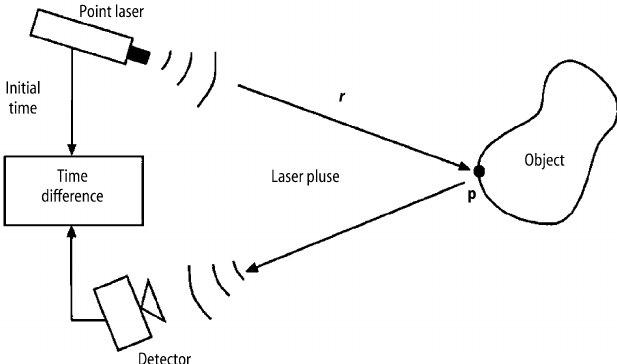
\includegraphics[scale=0.15]{pictures/polop2}
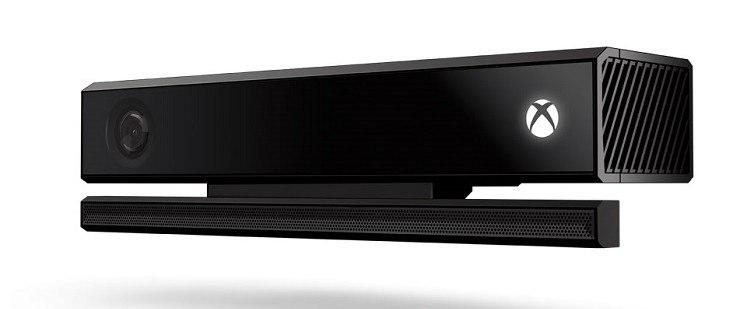
\includegraphics[scale=0.2]{pictures/polop1}
\end{figure}
Shortcomings:
\begin{itemize}
\item Low mapping rate (~30Hz)
\item Motion artifacts
\item Multipath-interference
\end{itemize}
\end{frame}


%%%%%%%%%%%%%%%%%%%%%%%%%%%%%%%%%%%%%%%
\begin{frame}{Structured Light}

Spatial patterns projected on the scene
\begin{figure}
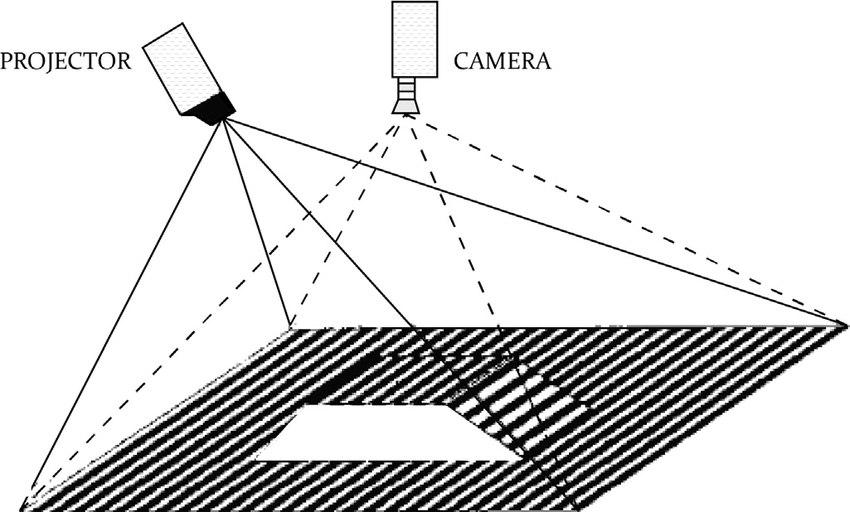
\includegraphics[scale=0.1]{pictures/polop4}
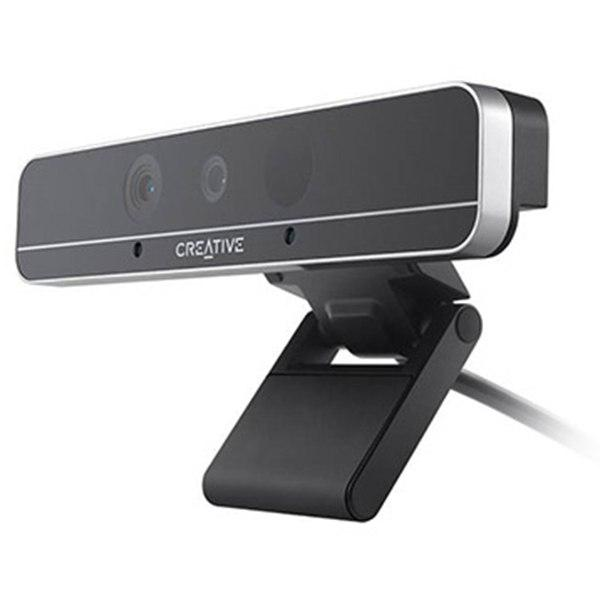
\includegraphics[scale=0.1]{pictures/polop3}
\end{figure}
Shortcomings:
\begin{itemize}
\item Robustness issues
\item Motion artifacts
\item Limited depth-range
\item Overlapping sensors cause interference
\end{itemize}
\end{frame}



%%%%%%%%%%%%%%%%%%%%%%%%%%%%%%%%%%%%%%%%

\begin{frame}{Active Stereo}

Using 2 calibrated cameras and 1 light source - solves a lot of the mentioned issues
\begin{figure}
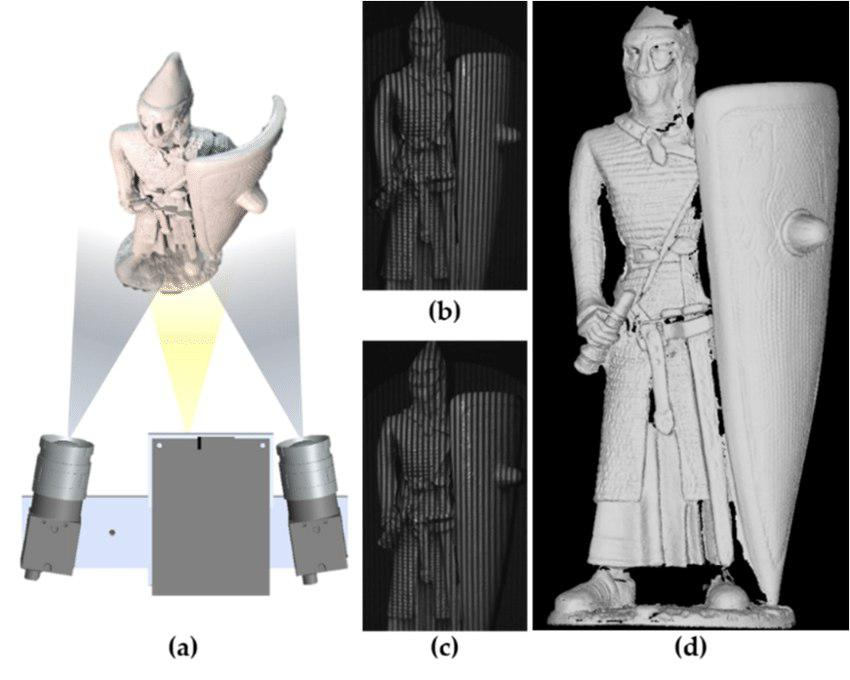
\includegraphics[scale=0.1]{pictures/polop5}
\end{figure}
\begin{itemize}
\item Mitigates multipath reflections
\item Improves robustness
\item Avoids interference between multiple systems
\item BUT correspondence search has high computational cost!
\end{itemize}

\end{frame}

